\documentclass[conference]{IEEEtran}
% \IEEEoverridecommandlockouts
% The preceding line is only needed to identify funding in the first footnote. If that is unneeded, please comment it out.
\usepackage{cite}
\usepackage{amsmath,amssymb,amsfonts}
\usepackage{algorithmic}
\usepackage{graphicx}
\usepackage{textcomp}

\def\BibTeX{{\rm B\kern-.05em{\sc i\kern-.025em b}\kern-.08em
    T\kern-.1667em\lower.7ex\hbox{E}\kern-.125emX}}

\usepackage{url}
\usepackage{comment}
\usepackage{listings}
\usepackage[usenames,dvipsnames,svgnames,table]{xcolor}
\graphicspath{{./figs/}} 
\usepackage{paralist}
\usepackage{hyperref}

\definecolor{dkgreen}{rgb}{0,0.6,0}
\definecolor{mauve}{rgb}{0.58,0,0.82}
\definecolor{light-gray}{gray}{0.88}

\lstdefinestyle{myPromela}
{frame=none,
  basicstyle=\ttfamily,
  language=Promela,
  aboveskip=1mm,
  belowskip=1mm,
  showstringspaces=false,
  columns=flexible,
  numbers=none,
  numberstyle=\tiny\color{gray},
  commentstyle=\color{dkgreen},
  stringstyle=\color{mauve},
  breaklines=false,
  breakatwhitespace=true,
  tabsize=2,
  linewidth=2\linewidth,
  morekeywords={always, eventually, until, implies, ltl}
}

\newcommand{\figref}[1]{Fig.~\ref{#1}}
\newcommand{\secref}[1]{Sec.~\ref{#1}}

\newcommand{\ie}{\textit{i.e.}}
\newcommand{\eg}{\textit{e.g.}}
\newcommand{\etal}{\textit{et al.}}
\newcommand{\etc}{\textit{etc.}}
\newcommand{\adhoc}{\textit{ad hoc}}
\newcommand{\phware}{PHware}

\newcommand{\scitesection}[1]{\section{\uppercase{#1}}}

\begin{document}

\title{
  Model Checking Functional Integration of Human Cognition and Machine Reasoning
}

\author{
\IEEEauthorblockN{Bryce Pierson}
\IEEEauthorblockA{\textit{Brigham Young University} \\
Provo UT, USA \\
\url{bryce.mckay.pierson@gmail.com}}
\and
\IEEEauthorblockN{Eric Mercer}
\IEEEauthorblockA{\textit{Brigham Young University} \\
Provo UT, USA \\
0000-0002-2264-2958}
}

\maketitle

\begin{abstract}
    \begin{comment}
Functional integration of human cognition and machine reasoning is an industry-wide problem where failure risks health or safety.
Differences in human versus machine functioning obscure conventional integration. 
We introduce cognitive work problems (CWP) for rigorous, verifiable functional integration. 
CWP specify the cognitive problem that integrated designs must solve. 
They are technology-neutral, abstract work objects, allowing people and computing to share and transform them in coordination.
The end-to-end method is illustrated on a system that employs AI for remote patient monitoring (RPM) during COVID-19 home care. 
The CWP specified \emph{actionable risk awareness} as the medical problem RPM must solve.
Graphical modeling standards enabled user participation: CWP as finite state machines and system behavior in BPMN. 
For model checking, the CWP’s logical content was translated to linear temporal logic (LTL) and the BPMN into Promela as inputs to the SPIN model checker. 
SPIN verified the Promela implements the LTL correctly.
We conclude this CWP-derived RPM design solves the medical problem and enhances patient safety. 
The method appears general to many critical systems.

\end{comment}

Many critical systems industry-wide demand fail-safe integration of human cognition and machine reasoning.
This integration is difficult because of inherent dissimilarity between human and machine functioning.
Existing methods for validating systems with human and machine functioning require expertise in formal verification and are labor intensive.
Additionally, error output from existing methods is exclusively text-based and demands extensive time and familiarity to comprehend.
We introduce a tool for automating verification of systems with human and machine functioning.
Participation in the automation process requires very little knowledge of the underlying model checking tools.
We demonstrate the effectiveness of the tool using examples of models including subtle-but-critical errors.
We present an extensible model to demonstrate the scalability of the automated verification tool.
We also introduce an understandable visual representation of model failures to enable quick iteration on subsequent model versions.
The visual representation is critical to understanding why a model doesn't comply with given temporal properties.
We conclude that model checking is a viable method for verifying systems that require human and machine integration.

\end{abstract}

\begin{IEEEkeywords}
    Cognitive Modeling, Business Process Modeling, Model Checking, Model-Based Validation, SPIN, Linear Temporal Logic, COVID-19
\end{IEEEkeywords}

\section{Introduction}
\begin{comment}

This paper introduces a new method of \emph{model based systems engineering} (MBSE) for functional integration and verification of joint human-computer teaming on cognitive tasks. 
The original contribution to integration is a specification of the abstract, cognitive work problem (CWP) the design must solve \cite{workcentered,BERRY201615,chi2010}, represented as a declarative, computation independent model \cite{Garrido}.
The technical neutrality of this cognitive model makes it a shareable object of abstract work which different types of actors can transform, despite vastly different performance properties.
Thus, a CWP provides the means to integrate the work of a distributed cognitive system that transforms a CWP from its initial state to the goal state required from the system.

The original contribution to design verification reuses the CWP as a new type of required property for model checking to prove the correctness of integrated designs.
The capability to integrate human cognition with machine reasoning and then verify design correctness can increase safety and reliability for a wide range of critical systems.

Our proof-of-technology is illustrated by a case-study of telehealth augmented by \emph{remote patient monitoring} (RPM).
Although telehealth has rapidly gained acceptance for improving accessibility \cite{Medicare} and reducing transmission rates \cite{10.1093/jamia/ocaa067} the remote and asynchronous context of telehealth also introduces risk that patients may deteriorate before physicians can be aware and intervene \cite{10.1097/ALN.0000000000003578}.
The experience of this integrated design process makes clear the difficulty of reasoning about even simple systems without a verification tool.

Bionous \phware\textsuperscript{\textregistered} is an application under development to enhance the telehealth safety of COVID-19 patients with RPM of their vital signs \cite{Phware}.
\phware\ measures and streams seven vital signs: temperature, oxygen saturation, respiration rate, pulse and its variability, and dia/systolic blood pressures.
A single \phware\ ring or finger-clip can be used at home to sense all vital signs in a 60-90 second session, and then send them to a smartphone via Bluetooth.
A smartphone app uploads the data to AI cloud services for storage and machine-learning to assign numerical values to vitals, analyze their trends, and send alerts.
A web-based dashboard displays the trends and alerts to provide clinicians with \emph{actionable risk awareness} of their outpatients.
The streaming of vital signs and alerts serve as an early warning system to maintain clinicians’ awareness and prioritize their attention, thereby enhancing home care safety.

The following section defines \emph{actionable risk awareness} as the CWP for \phware, developed with clinicians and other experts \footnote{Ann Marie Kimball, an internationally recognized MD epidemiologist in emerging infectious disease, provided medical advice}.
\secref{sec:ltl} details translation of the CWP into \emph{Linear Temporal Logic} (LTL) \cite{10.5555/975331} properties that exactly capture the meaning of the CWP and are suitable for use with a model checker.
%LTL is a first-order predicate calculus with the ability to reason about the temporal ordering of events \cite{10.5555/975331}.
%Any viable design for vital sign RPM of COVID-19 patients must verify against each LTL property created from the CWP in order to claim it takes appropriate action relative to patient risk.
\secref{sec:workflow} presents the \phware\ workflow model in the \emph{Business Process Modeling Notation} (BPMN) \cite{BPMN} that integrates the activities of clinicians, AI cloud services, and patient-caregivers.
\secref{sec:bpmn} details the translation of the workflow into an equivalent \emph{Process Meta-language} (Promela) model for the SPIN model-checker \cite{spin} with \secref{sec:env} discussing how the inputs to the workflow are defined.
The results of the SPIN verification are given in \secref{sec:results}.

The original finite state model, the BPMN model, and full Promela model, with the LTL properties for the CWP, are in a public Github repository \cite{repo}.
The \texttt{README.md} file summarizes its content and how to use SPIN to verify the model.
Figure titles in the electronic version of this manuscript link to equivalent, but larger, more legible versions in GitHub.


% The intentions of the detailed case study are to show the viability of augmenting workflows with CWP for functional integration and model checking, and to illustrate the value for automated reasoning in any design environment.
% SPIN worked effectively and efficiently in this project in terms of performance and iterative design analysis.
% The workflows and CWP revisions were easy to verify when posted, and when SPIN found violations, the accompanying counter-examples provided critical insights to the unexpected, and often overlooked, outcomes common in asynchronous interactions.
% These insights were absolutely necessary for those working on the workflows and those working on the CWP to arrive at the presented final forms.
% The experience of this integrated design process with the model checker makes clear that it is difficult to reliably reason about even simple concurrent systems without a verification tool.
\end{comment}

This paper introduces a novel approach to automating model checking of systems involving integration of human cognition and machine reasoning. We build upon prior work \cite{mercer22} introducing a new method for \emph{model based systems engineering} (MBSE) . A core component to functional integration is an abstract specification of work, a Cognitive Work Problem (CWP). A CWP is a computation-agnostic model, allowing it to be operated on by any actor, regardless of their performance properties. The work in a distributed cognitive system is integrated if it transforms a CWP from its initial state to a goal state.

Humans and machines work together in practically every field. In may of these fields, seamless integration is not only desired, but critical. There are safety concerns, such as in aeronautics\cite{aeronautics1, aeronautics2} or healthcare\cite{healthcare1, healthcare2}. There are financial concerns, such as in banking\cite{banking1,banking2}. There are even concerns about integrity, such as in voting\cite{voting1, voting2}.
\egm{Add citations to the above text justify the claims where possible. Keith may have such citations or they may exist in the paper that first introduces the translation.}

This work progresses the path toward seamless integration between humans and machines in business processes. It does that by partially automating a process which allows Business Process Model and Notation (BPMN)\cite{BPMN} models to be verified against the CWP, a separate model which is taken as ground truth. The CWP has two parts, an object state and a state machine; the former connects it to the BPMN workflow model. The goal of the verification process is to ensure that the BPMN workflow can manipulate the object state toward any of the final states specified by the CWP state machine. Verification must also ensure that the BPMN workflow uses only allowed transitions to reach a final state. So that the process may benefit human-computer interaction, it is critical that the CWP should not reason about the environment in which the work gets done, the context in which the work gets done, or the actors who perform the work.
\egm{BPMN needs to be defined. Also, make clear that the separate model is the CWP. It may also be wise to refer to what makes up a CWP, object state and a state machine, and how the CWP and workflow are related to one another by virtue of that object state. The goal or the workflow is to evolve the object state to any of the allowed final states in a ways that always follows transitions allowed by the CWP.}

Verification of functional integration has been attempted before using task decomposition \cite{decomposition}. There are also examples verifying properties of BPMN workflows.\cite{bpmnVerification1, bpmnVerification2, ASMverification} These methods verify properties such as absence of deadlock, fair resource usage, and absence of invalid end states.
As mentioned earlier, this work is primarily built upon the work in \cite{mercer22}, which creates a foundation for functional integrity of human cognition and machine reasoning using model checking. Our work borrows much of the structural designs of both Linear Temporal Logic (LTL)\cite{ltl} property generation and also Process Meta-Language (Promela)\cite{promelaManual} model generation, while adding automation and counterexample visualization.
Prior work in verifying BPMN models can verify certain global properties, such as absence of deadlock or the existence of an end state, but this work adds a ground truth model which introduces verification of the semantics of the BPMN model as well as the structure. 
\egm{This paragraph needs to expand, and actually cite, the related work. There is work on task decomposition as a way to do functional integration. There is my work with Keith that is published that must be discussed here since this paper needs to be precise about what it does new, or what problems my previous paper left unsolved (automation and counter-example explanation). There is also work on verifying BMPN message diagrams with SPIN and some work on verifying mode confusion on graphical interfaces. There should be maybe two paragraphes here: the first is related stuff with other ways to do functional integration and the second is my work that is better than that in the first paragraph but still leaves unsolved automation and counter-example explanation.}

\egm{Missing is a clear statement about our new solution to the problem and what it is that that solution accomplishes that my prior work does not do. It should also state how we intend to show that our new solution works and solves the problems that it claims to solve. After that paragraph, add a paragraph that list the contributions of the research discussed in this paper.}

\secref{sec:simpleExample} provides a simple example of a BPMN-CWP pair and shows how model checking can allow us to prove correct implementation.
\secref{sec:background} gives a background of \cite{mercer22} and how it relates to the work in this paper.
\secref{sec:automaticGeneration} looks at the difficulties of automating the Promela generation.
\secref{sec:counterexample} introduces the counterexample visualization tool, which improves significantly on the prior methods of debugging BPMN workflow errors.
\secref{sec:eval} provides evaluation characteristics, as well as the set of examples this tool is evaluated on, explaining the unique aspects of each example, as well as providing performance statistics.

\section{Background}
\label{sec:background}
\egm{You are part of the proposal overleaf project where I am trying to write formal digests of my previous work. Let's plan to revise, refine, and add to what is there. That will be the basis for this background section. Missing in the text I have written is a clear mathematical statement of the CWP and the same for the BPMN. I might suggest that we create subsections here for the CWP and the BPMN with each containing the definitions and the associated translations. The goal of this section is then to define the CWP, with its LTL interpretation, and define the BPMN (workflow) with its Promela interpretation.}

The work in \cite{mercer22} accomplishes a few things that are necessary background components for this work. First, it introduces a method for translating a BPMN diagram into verifiable Promela code. Second, it introduces a way of interpreting a CWP as a set of LTL properties and defines this method rigorously. Lastly, it uses a practical example in healthcare to show that the Promela and LTL can be used together to verify the integration of human and machine cognition in the original BPMN.

These processes are applied to a medical practice centered around a device for at-home COVID-19 care. The results showed that the process verified against a provided CWP and therefore, integrated the human and machine actors correctly.

\section{BPMN Translation Automated Reasoning}
\label{sec:bpmnReasoning}
\egm{There needs to be a section on the automatic translation of the CWP to the LTL properties. There the expression language should matter as well as the object state: where and how it is defined.}

\egm{I might suggest grouping this section and the next into a single section titled: Automatic Generation of the Promela Model. The opening paragraph should list the interesting challenges for which we provide interesting solutions. Each of those should be it's own sub-section. The environment generation is one such challenge.}
Automating the BPMN-to-Promela is not trivial. There are multiple implied semantics in BPMN that make it difficult. For example, parallel gateways are a node in BPMN semantics that indicates the parallel execution of multiple branches. However, the exact same node is used to both fork these branches and to join them. Reasoning about the structure of the BPMN is then necessary to understand exactly how a parallel gateway node should behave in Promela. This logic is also applicable in some ways to XOR gateway nodes.

Additionally, it is necessary to understand which text in the BPMN is flavor text, contributing to the readability, and which text is to be interpreted as conditions. In this project, flows coming out of XOR and complex gateways must be equality or inequality conditions, unless the gateway is acting as a join of multiple branching possibilities as discussed in the previous paragraph.


\section{Environment Construction}
\label{sec:envConstruction}
\egm{The need for an environment is yet discussed. It should be made very clear in the background on the BPMN translation. Indeed, a major pain point in my work was the environment. What should it be? How should it be? I spent a ton of time on the different behavior models. Also, the diagram, Fig. 8, talks about Behavior Models and not environment. I suggest to adopt Behavior Model everywhere and dump the notion of environment altogether. Or, adopt environment and dump behavior model everywhere. In any case, I'm not sure breaking it out in its own section makes sense unless it is framed before in the context of the translation algorithm. In any case, it needs to be better integrated with the BPMN translation. Without that context, it's hard to understand what is going on.}

Another difficult part of automating is the generation of an environment. The initial definition of the environment must be provided to the automation tool as a set of variables and constants. Every variable that shows up in a conditional edge in the BPMN must be defined at this stage, otherwise verification will cease.

The object state is currently defined in a TXT file. An example of an object state file is given below.
%
{\small
\begin{lstlisting}[style=myTXT]
const enum belowPaymentAmount belowPaymentAmount
const enum paymentAmount paymentAmount
const enum INIT INIT
const enum other other
const enum buyerName buyerName
const enum sellerName sellerName
const enum agreed agreed
const enum failed failed
const enum pending pending
const enum noRetry noRetry

enum terms terms pending [agreed, failed, pending, noRetry]
enum backpackOwner backpackOwner sellerName [buyerName, sellerName]
enum paymentOwner paymentOwner buyerName [sellerName, buyerName]
enum paymentOffered paymentOffered pending [paymentAmount, belowPaymentAmount, pending, noRetry]
\end{lstlisting}
}
%
The first thing defined are the constants. You will notice that each constant is stated twice in the given example. The first is the name of the constant in the CWP and the second is the name of the constant in the BPMN. When the BPMN and CWP are created synchronously, as in this example, coordinating the names precisely made sense. But we acknowledge that this may not always be possible or desirable.

Despite not being explicitly stated, "True" and "False" are always included as constants. 

Possible data types are "enum", "byte", "short", and "int".
After two line breaks, the file begins defining the object state variables. For each variable, both the CWP name and BPMN name are listed first, followed by the initial value. Then, in square brackets, the set of assignable values is listed.

It should be noted that initial variable values are essential for the verification process. This is because the verifier will first check the LTL property, then step forward in the Promela code.

\egm{Does there need to be a section on model checking in the backgroud where these type of details are defined and discussed? Also, while it's an interesting point, is it a necessary point? Is it enough to just state that every part of the object state, and extended BPMN state, needs an initial value? These values define the initial starting state of the BPMN and CWP?}

This means that variables cannot be initialized in the first activity of the BPMN unless uninitialized variables are accounted for in the CWP. We recommend avoiding this and declaring initial values for at least some of the environment variables.

Another important point is that the ordering of constants matters. In promela, mtype variable options are assigned integer values under the hood. For checking equality and inequality, this doesn't matter. But it does matter when doing a comparison. In Face2Face, one condition for a successful purchase is that \lstinline[style=myPromela]{paymentOffered < paymentAmount}. 
\egm{Didn't our example get a name, and didn't we say we would refer to it by that name? I might suggest using the name. Thus far, we haven't used the example to much either in automation section.}
To assist in asserting this comparison, two constants are added to the object state definition: 
\lstinline[style=myPromela]{paymentAmount}
and \lstinline[style=myPromela]{belowPaymentAmount}. 
It is critical that \lstinline[style=myPromela]{belowPaymentAmount} 
be declared before \lstinline[style=myPromela]{paymentAmount} so that the underlying integer value is indeed lesser.

\egm{OK. The above is a big deal. This type of subtly and nuance I think is very problematic. The object state consists of only `mtype` but we are allowing the full range of operators on that type including relational operators? That seems really dangerous. Right? Why not allow, for example, variables with primitive types, so the object state can have a `temperature` value that is a `short`? In any case, I suggest a new section be added at the beginning of the automation section that discusses nothing but the object state definition and its implications on writing expressions.}

These environment variables are manipulated during the activities in the BPMN. The exact nature of these manipulations plays a vital role in the verification process. We call these manipulations the behavior models.

The behavior models are defined in a Promela (PML) file. This is an example snippet from a behavior models file:
%
{\small
\begin{lstlisting}[style=myPromela]
//Start7
inline Start7_BehaviorModel(){
	skip
}
//T1
inline T1_BehaviorModel(){
	if
		:: true -> backpackOwner = sellerName
	fi
	if
		:: true -> paymentOwner = buyerName
	fi
	updateState()
}
//XOR1
inline XOR1_BehaviorModel(){
	skip
}
//T2
inline T2_BehaviorModel(){
	if
		:: true -> terms = agreed
		:: true -> terms = failed
	fi
	if
		:: true -> paymentOffered = paymentAmount
		:: true -> paymentOffered = belowPaymentAmount
	fi
	updateState()
}
\end{lstlisting}
}
%
The PML file must contain a valid PML inline for each activity in the BPMN diagram. These inlines will be called when a token passes through an activity in the Promela model. For example, \lstinline[style=myPromela]{T1_BehaviorModel()}
is the name of the inline that will be executed when the task named \lstinline[style=mypromela]{T1} 
is reached. If the file does not exist when the translation process begins, the automation tool will output a stub file with the skeleton of each inline defined.
\egm{I assume the translation tool will never overwrite the file? Always a concern...}
Next the user must add Promela code to manipulate the object state in a way that is consistent with the intended behavior of the business process.  The inlines, in many cases, should contain nondeterminism. Using this nondeterminism, every reasonable outcome of that activity will be considered during verification. The creation of the behavior models is one aspect of translation that still requires an expert in model checking to complete. The writer of the Promela inlines must not only be proficient in the model checking language, but must also understand the nondeterministic intentions of the inlines.
\egm{Missing is a discussion of on of the behavior models in the code snippet? We have the face2face example, add text that talks about the code in that example. What does it mean? What is the implication? That might help understand the role, and need, for the non-determinism. Right?}



\section{Counterexample Visualization}
\label{sec:counterexample}
Automated model verification is only useful to us as far as the generated counterexamples are comprehensible. Without comprehensible counterexamples, the negative verification results provide very little or no insight into the source of the error. The fairness constraint used in this project introduces an issue into the counterexamples. Because the fairness property is a prerequisite for every other property, the execution error trails must end in a valid end state. This means that regardless of where an error actually occurs, the trail will always continue until the valid end state is reached. Therefore, at first glance, there is a chance that many error trails will look very similar (or even identical) to each other. The tool explained in this section aims to assist the user in both identifying the moment(s) of failure for each counterexample and also uniquely identify each error trail.

The error visualizer is a mechanism to visualize both the workflow and the CWP as they evolve along the error trace. This allows the user to identify the moment the CWP was violated and examine the history preceding the error. A set of annotated images are generated for both the workflow and CWP. Each annotated image corresponds to a single step of execution during the verification process. A step is characterized by the execution of an element in the BPMN. The execution of each element initiates another step in the counterexample. \figref{fig:ErrorVisualizationRoadmap} shows the high-level process of generating the error visualization output. 

\begin{figure*}[t]
  \begin{center}
    \begin{tabular}{c}
        \frame{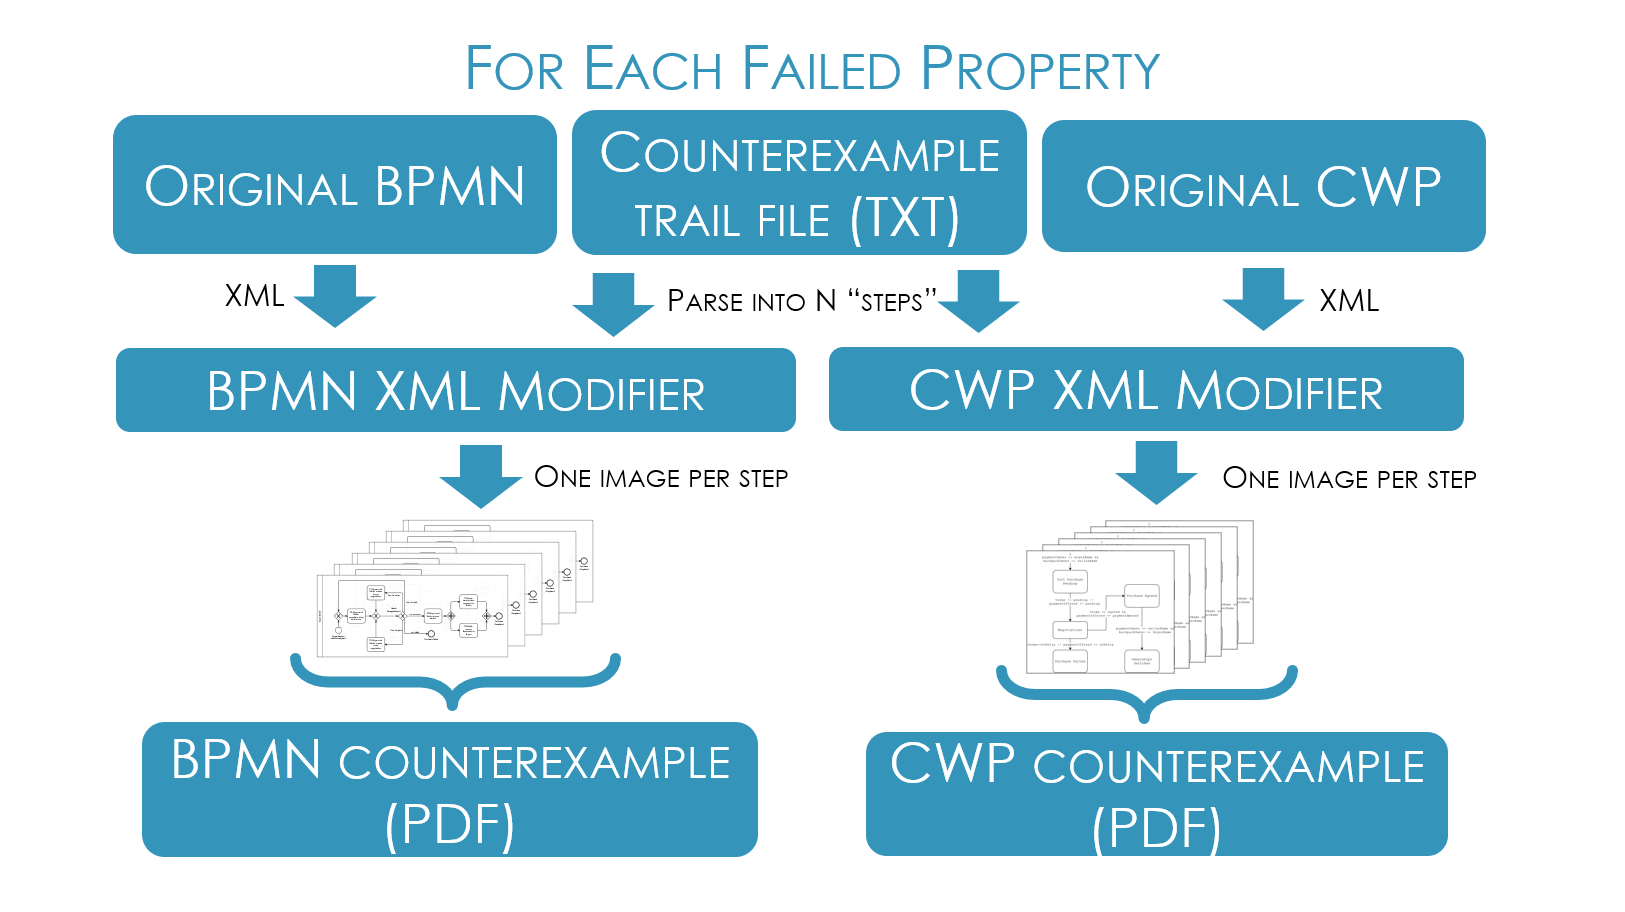
\includegraphics[width=\textwidth]{../figs/Other/ErrorVisualizationRoadmapWhiteBG.png}}
    \end{tabular}
  \end{center}
\caption{Error Visualization Generation Pipeline}
\label{fig:ErrorVisualizationRoadmap}
\end{figure*}


An example annotated BPMN image for step 1 is shown in \figref{fig:ErrorVisualizationBPMN} and the corresponding CWP is shown in \figref{fig:ErrorVisualizationCWP}. Step 1 is the initial step where the start event is executed and the token moves toward the first XOR gateway.

\begin{figure*}[t]
  \begin{center}
    \begin{tabular}{c}
        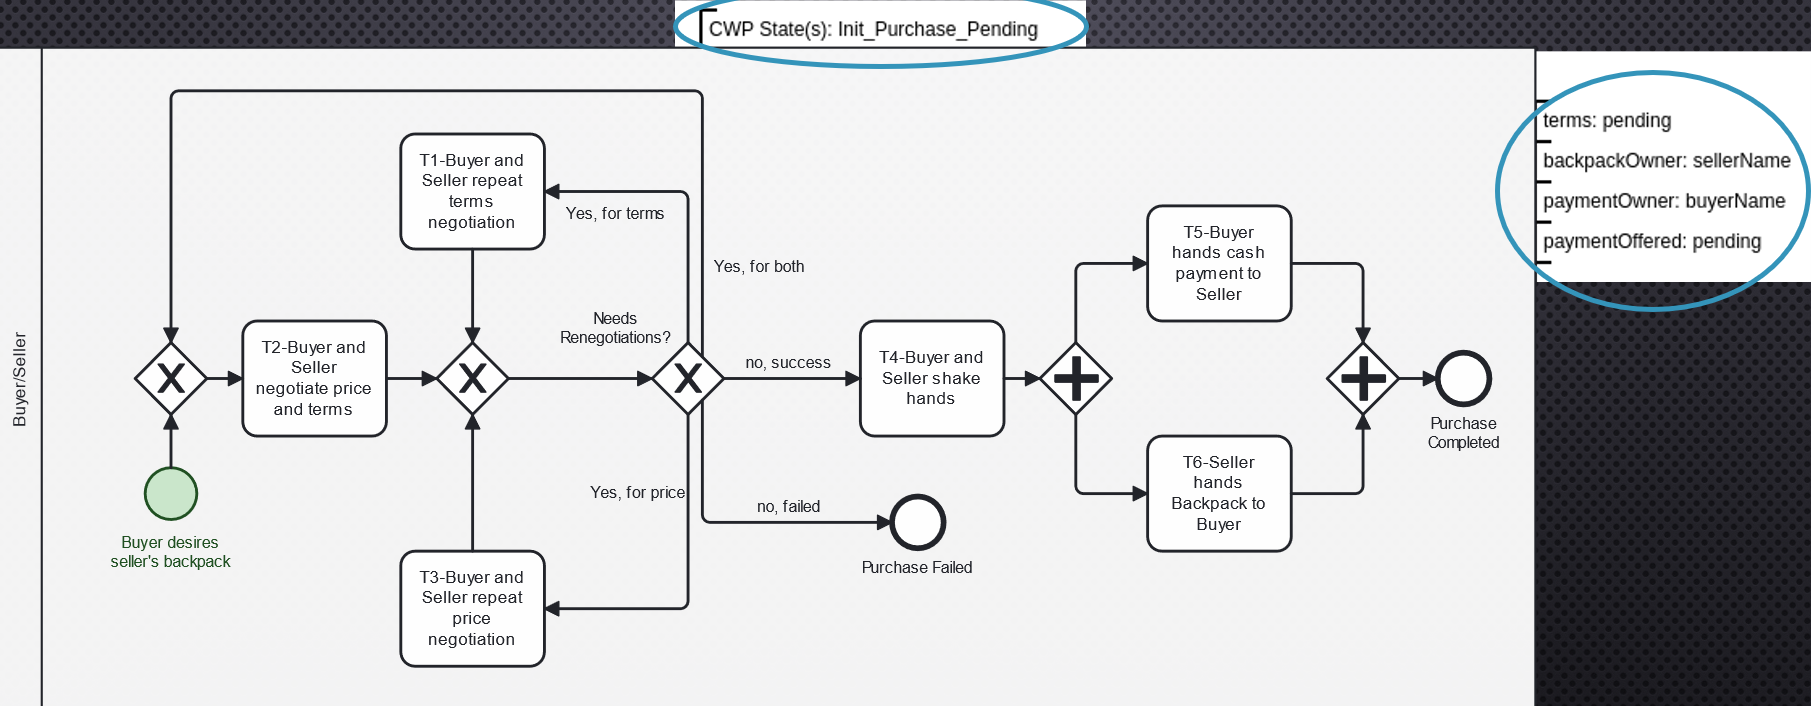
\includegraphics[width=\textwidth]{../figs/Other/ErrorVisualizationBPMN.png}
    \end{tabular}
  \end{center}
\caption{Annotated BPMN for the first step of an error in Face2Face}
\label{fig:ErrorVisualizationBPMN}
\end{figure*}


\begin{figure*}[t]
  \begin{center}
    \begin{tabular}{c}
        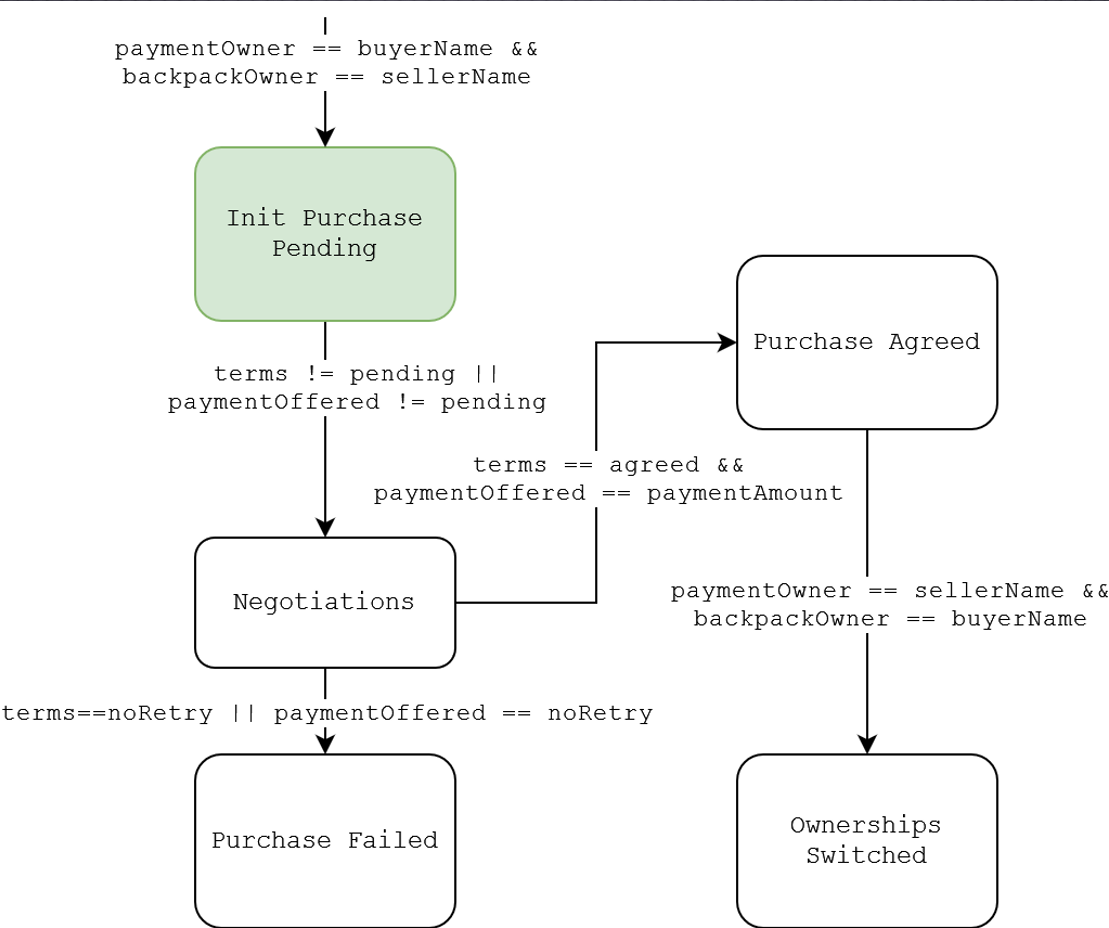
\includegraphics[width=\textwidth]{../figs/Other/ErrorVisualizationCWP.png}
    \end{tabular}
  \end{center}
\caption{Annotated CWP for the first step of an error in Face2Face}
\label{fig:ErrorVisualizationCWP}
\end{figure*}

Aside from the path of execution, there are several notable annotations, particularly on the BPMN. First, at the top of the BPMN workflow, there is a list of the state(s) in which the BPMN currently resides. This is important to pay attention to because it will show precisely when a property is violated. For example, if any "mutex" property is violated, there will eventually be a step in execution that lists multiple states at the top of the image. This moment is the moment of failure. Additionally, if the "alwaysInAState" property fails, there will eventually be a step in which no states are listed.

Next, in the top right corner of the BPMN workflow, each of the object state variables are listed, along with their current values. This information can help a user find subtle errors involving CWP edge labels, BPMN behavior models, and more. Each variable is highlighted if its value is changed after the current BPMN step is finished.

To assist with distinguishing similar or identical trails, an annotation is included in the top center that indicates possible moments of interest for the specific property in question. This feature indicates moments where the underlying LTL property takes a step (meaning that something interesting happened in regards to the logical expressions referenced in the property.)

Finally, the CWP image is annotated by coloring the current state(s). If the BPMN only resides in one state, it is colored green. If the BPMN resides in multiple states simultaneously, they will be colored red. Additionally, if on the previous step, the BPMN resided in a state from which there is not a transition to the current state, the current state will be colored red.

It is important to note that the visualizer shows the BPMN first taking a step, followed by the CWP updating. Therefore, the annotated CWP image associated with step $n$ indicates that the corresponding BPMN resides in the colored state(s) after it has taken its $n$th step. The state annotation and the object state variables annotation on the BPMN image also represent the object state \emph{after} the BPMN takes its step.

The counterexample visualizer currently has limitations in regards to existential properties. An existential property is one that is proven by finding a witness - a trail that shows some state exists in the model. A witness is manifest as an error in SPIN, but the absence of a witness means the property failed to verify. In this case, the counterexample visualizer has nothing to report, except that a witness was not found. More informative reporting of these cases is a difficult question that is left for future work.


\section{Evaluation}
\label{sec:eval}
This tool has been used to verify five BPMN-CWP pairs. The effectiveness of this tool will be measured by both the verification time. Two procedural generated, scalable examples will be used to measure both sequential (many linear decisions) and parallel (many synchronous actors) scalability of this model checking approach.

The first example has been explained thoroughly in \secref{sec:simpleExample}. The rest of the examples will be destribed in this section, along with tables and graphs of results.

\begin{comment}
\figref{fig:face2face_bpmn} shows the BPMN of the first example, a face-to-face purchase. The Buyer and seller are condensed into a single actor for simplicity in this model. The purchase process involves negotiation periods for both the price and the terms. Once the price and terms are agreed upon, the model can proceed to the exchange and then exit. \figref{fig:purchase_cwp} shows the CWP for this purchase. The CWP has 5 states, of which 2 are goal states. It is the workflow's responsibility to either send the state of the CWP to "Purchase Failed" or to "Ownerships Switched". Note that even though "Purchase Failed" might not sound like a goal state, it is for purposes of verifying eventual termination.
\end{comment}

\egm{There needs to be discussion, at the beginning, that gives an overview of the evaluation in terms of what it is trying to show and how it goes about showing that. The reader then understands why each of the example is included and discussed. What measures are we going the show with each example? Verification time? Model development time? Model size? I'm not sure what is of value.}

\figref{fig:buynsell_bpmn} shows the BPMN of the second example, a remote purchase system named "BuyN'Sell". This BPMN model is similar to the example in \secref{sec:simpleExample} except that it splits the buyer and seller into different parties, as well as introduces some reasoning about fulfillment of the order. BuyN'Sell shares a CWP with the previous example, shown in \figref{fig:purchase_cwp}. This example was chosen to show the versatility of CWP. Because it shouldn't reason at all about the context or the actors in the work, it can be used to verify multiple BPMN diagrams involving an exchange of goods, even though they may have drastically different performance characteristics.

\begin{figure*}[t]
  \begin{center}
    \begin{tabular}{c}
        \includesvg[inkscapeformat=png, width=\textwidth]{../figs/BPMN/buynsell_Mar_27_2023_workflow.svg}
    \end{tabular}
  \end{center}
\caption{BPMN workflow for remote purchase example, BuyN'Sell}
\label{fig:buynsell_bpmn}
\end{figure*}

\figref{fig:phware_bpmn} shows the BPMN of the third example, the original example from \cite{mercer22}. In this example, a patient diagnosed with COVID-19 is being monitored remotely. \figref{fig:phware_cwp} shows the corresponding CWP. When we verify the BPMN against this CWP, we are ensuring that the patient is never incidentally mistreated in the BPMN according to the readings from the remote monitoring device. The initial example shows a single actor with branching paths. The second example shows multiple actors with mostly linear paths. This is the most complicated example so far, containing both multiple actors and branching paths.

\begin{figure*}[t]
  \begin{center}
    \begin{tabular}{c}
        \includesvg[inkscapeformat=png, width=\textwidth]{../figs/BPMN/phware_May_5_workflow.svg}
    \end{tabular}
  \end{center}
\caption{BPMN workflow for PHware example}
\label{fig:phware_bpmn}
\end{figure*}

\begin{figure*}[t]
  \begin{center}
    \begin{tabular}{c}
        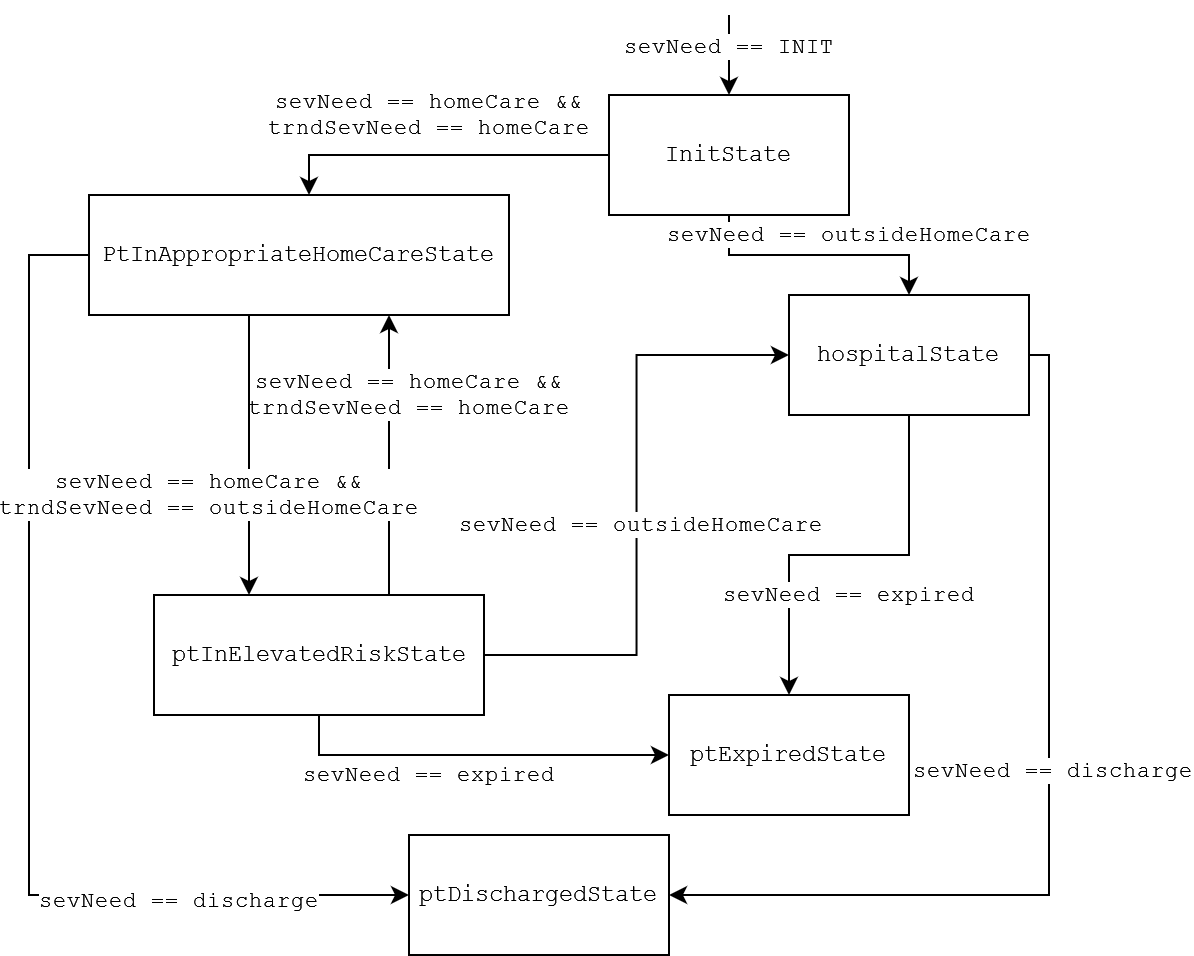
\includegraphics[width=\textwidth]{../figs/CWP/phware_CWP.png}
    \end{tabular}
  \end{center}
\caption{CWP state diagram for PHware example}
\label{fig:phware_cwp}
\end{figure*}

\figref{fig:longScaling2_bpmn} shows the BPMN of the fourth example. In this example, we show the scalability of the automation and verification process. This example contains a single actor with multiple decisions to make sequentially. We call this horizontal scaling. In this example, there are two sequential decisions. This number can be increased to push the limits of model checking in this context. \figref{fig:longScaling2_cwp} shows the corresponding CWP. The CWP here has just two states, only requiring that the BPMN execute to completion.

\begin{figure*}[t]
  \begin{center}
    \begin{tabular}{c}
        \includesvg[inkscapeformat=png, width=\textwidth]{../figs/BPMN/longScaling2_workflow.svg}
    \end{tabular}
  \end{center}
\caption{BPMN workflow for sequential scaling with two loops}
\label{fig:longScaling2_bpmn}
\end{figure*}

\begin{figure*}[t]
  \begin{center}
    \begin{tabular}{c}
        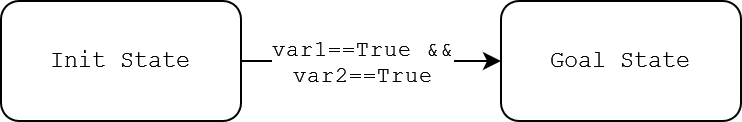
\includegraphics[width=\textwidth]{../figs/CWP/longScaling2_CWP.png}
    \end{tabular}
  \end{center}
\caption{CWP state diagram for sequential scaling with two loops}
\label{fig:longScaling2_cwp}
\end{figure*}

\figref{fig:wideScaling3_bpmn} shows the BPMN of the fifth example. This is also an example to show scalability. In this example, there are multiple actors, all with a single decision to make. In order to move throughIt is important to note that all of the actors interact with a single global state variable here. This type of scaling we will call vertical scaling. In this example, there are three actors \figref{fig:wideScaling3_cwp} shows the CWP for this example. Similar to the previous example, the CWP here only has two states. This ensures that each actor executes to completion.

\begin{figure*}[t]
  \begin{center}
    \begin{tabular}{c}
        \includesvg[inkscapeformat=png, width=\textwidth]{../figs/BPMN/wideScaling3_workflow.svg}
    \end{tabular}
  \end{center}
\caption{BPMN workflow for parallel scaling with three actors}
\label{fig:wideScaling3_bpmn}
\end{figure*}

\begin{figure*}[t]
  \begin{center}
    \begin{tabular}{c}
        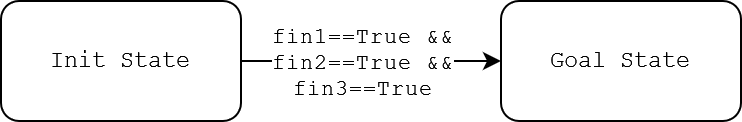
\includegraphics[width=\textwidth]{../figs/CWP/wideScaling3_CWP.png}
    \end{tabular}
  \end{center}
\caption{CWP state diagram for parallel scaling with three actors}
\label{fig:wideScaling3_cwp}
\end{figure*}

\figref{fig:verificationTimes} shows how long each model took to complete verification. Being the most simple example with no parallelism, the Face2Face verified the quickest, finishing in about two and a half minutes. The original Face2Face, with an error present, took slighly less time to verify. This is because, when the model checker detects an error, verification for a property can end sooner. If no errors are present, the entire state space must be searched. Next, BuyN'Sell, which introduces parallel execution, verified in four minutes and forty-one seconds. Finally, Phware, being the largest and most complex model, took eight minutes and forty-five seconds to verify.

\begin{figure*}[t]
  \begin{center}
    \begin{tabular}{c}
        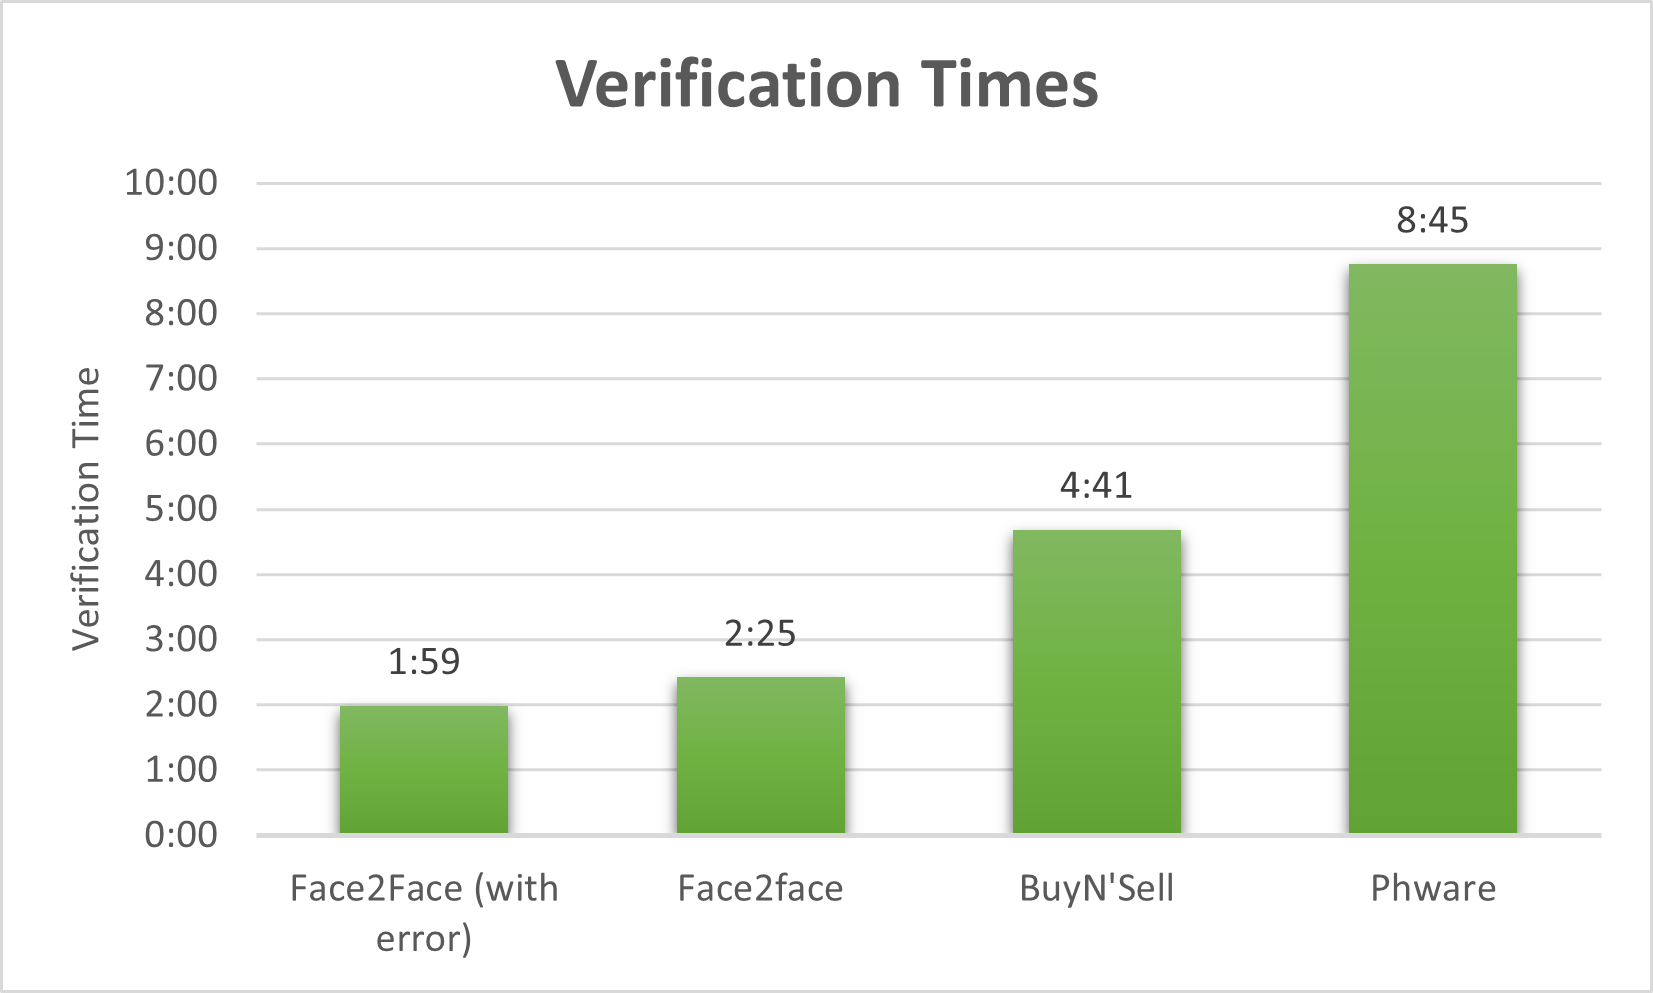
\includegraphics[width=\textwidth]{../figs/Data/Verification_Times.png}
    \end{tabular}
  \end{center}
\caption{Verification times for the four practical examples}
\label{fig:verificationTimes}
\end{figure*}

\figref{fig:longScalingVerificationTimes} shows the increase in verification time as the number of linear decisions increases in the sequential scaling BPMN example. The time requirement increases quadratically as the number of decisions increases. The largest example we tested had twenty sequential steps and took just over seven minutes to complete verification.

Several official BPMN best practice recommendations from BPM companies such as Camunda and Bizagi encourage BPMN modellers to keep diagrams as compact and simple as possible. If a model gets too large, it becomes difficult to read and understand. In those situations, it is best to identify parts of the model that can be separated into separate processes. Because of these recommendations, we believe that this model checking method scales sufficiently in sequential decisions.

\begin{figure*}[t]
  \begin{center}
    \begin{tabular}{c}
        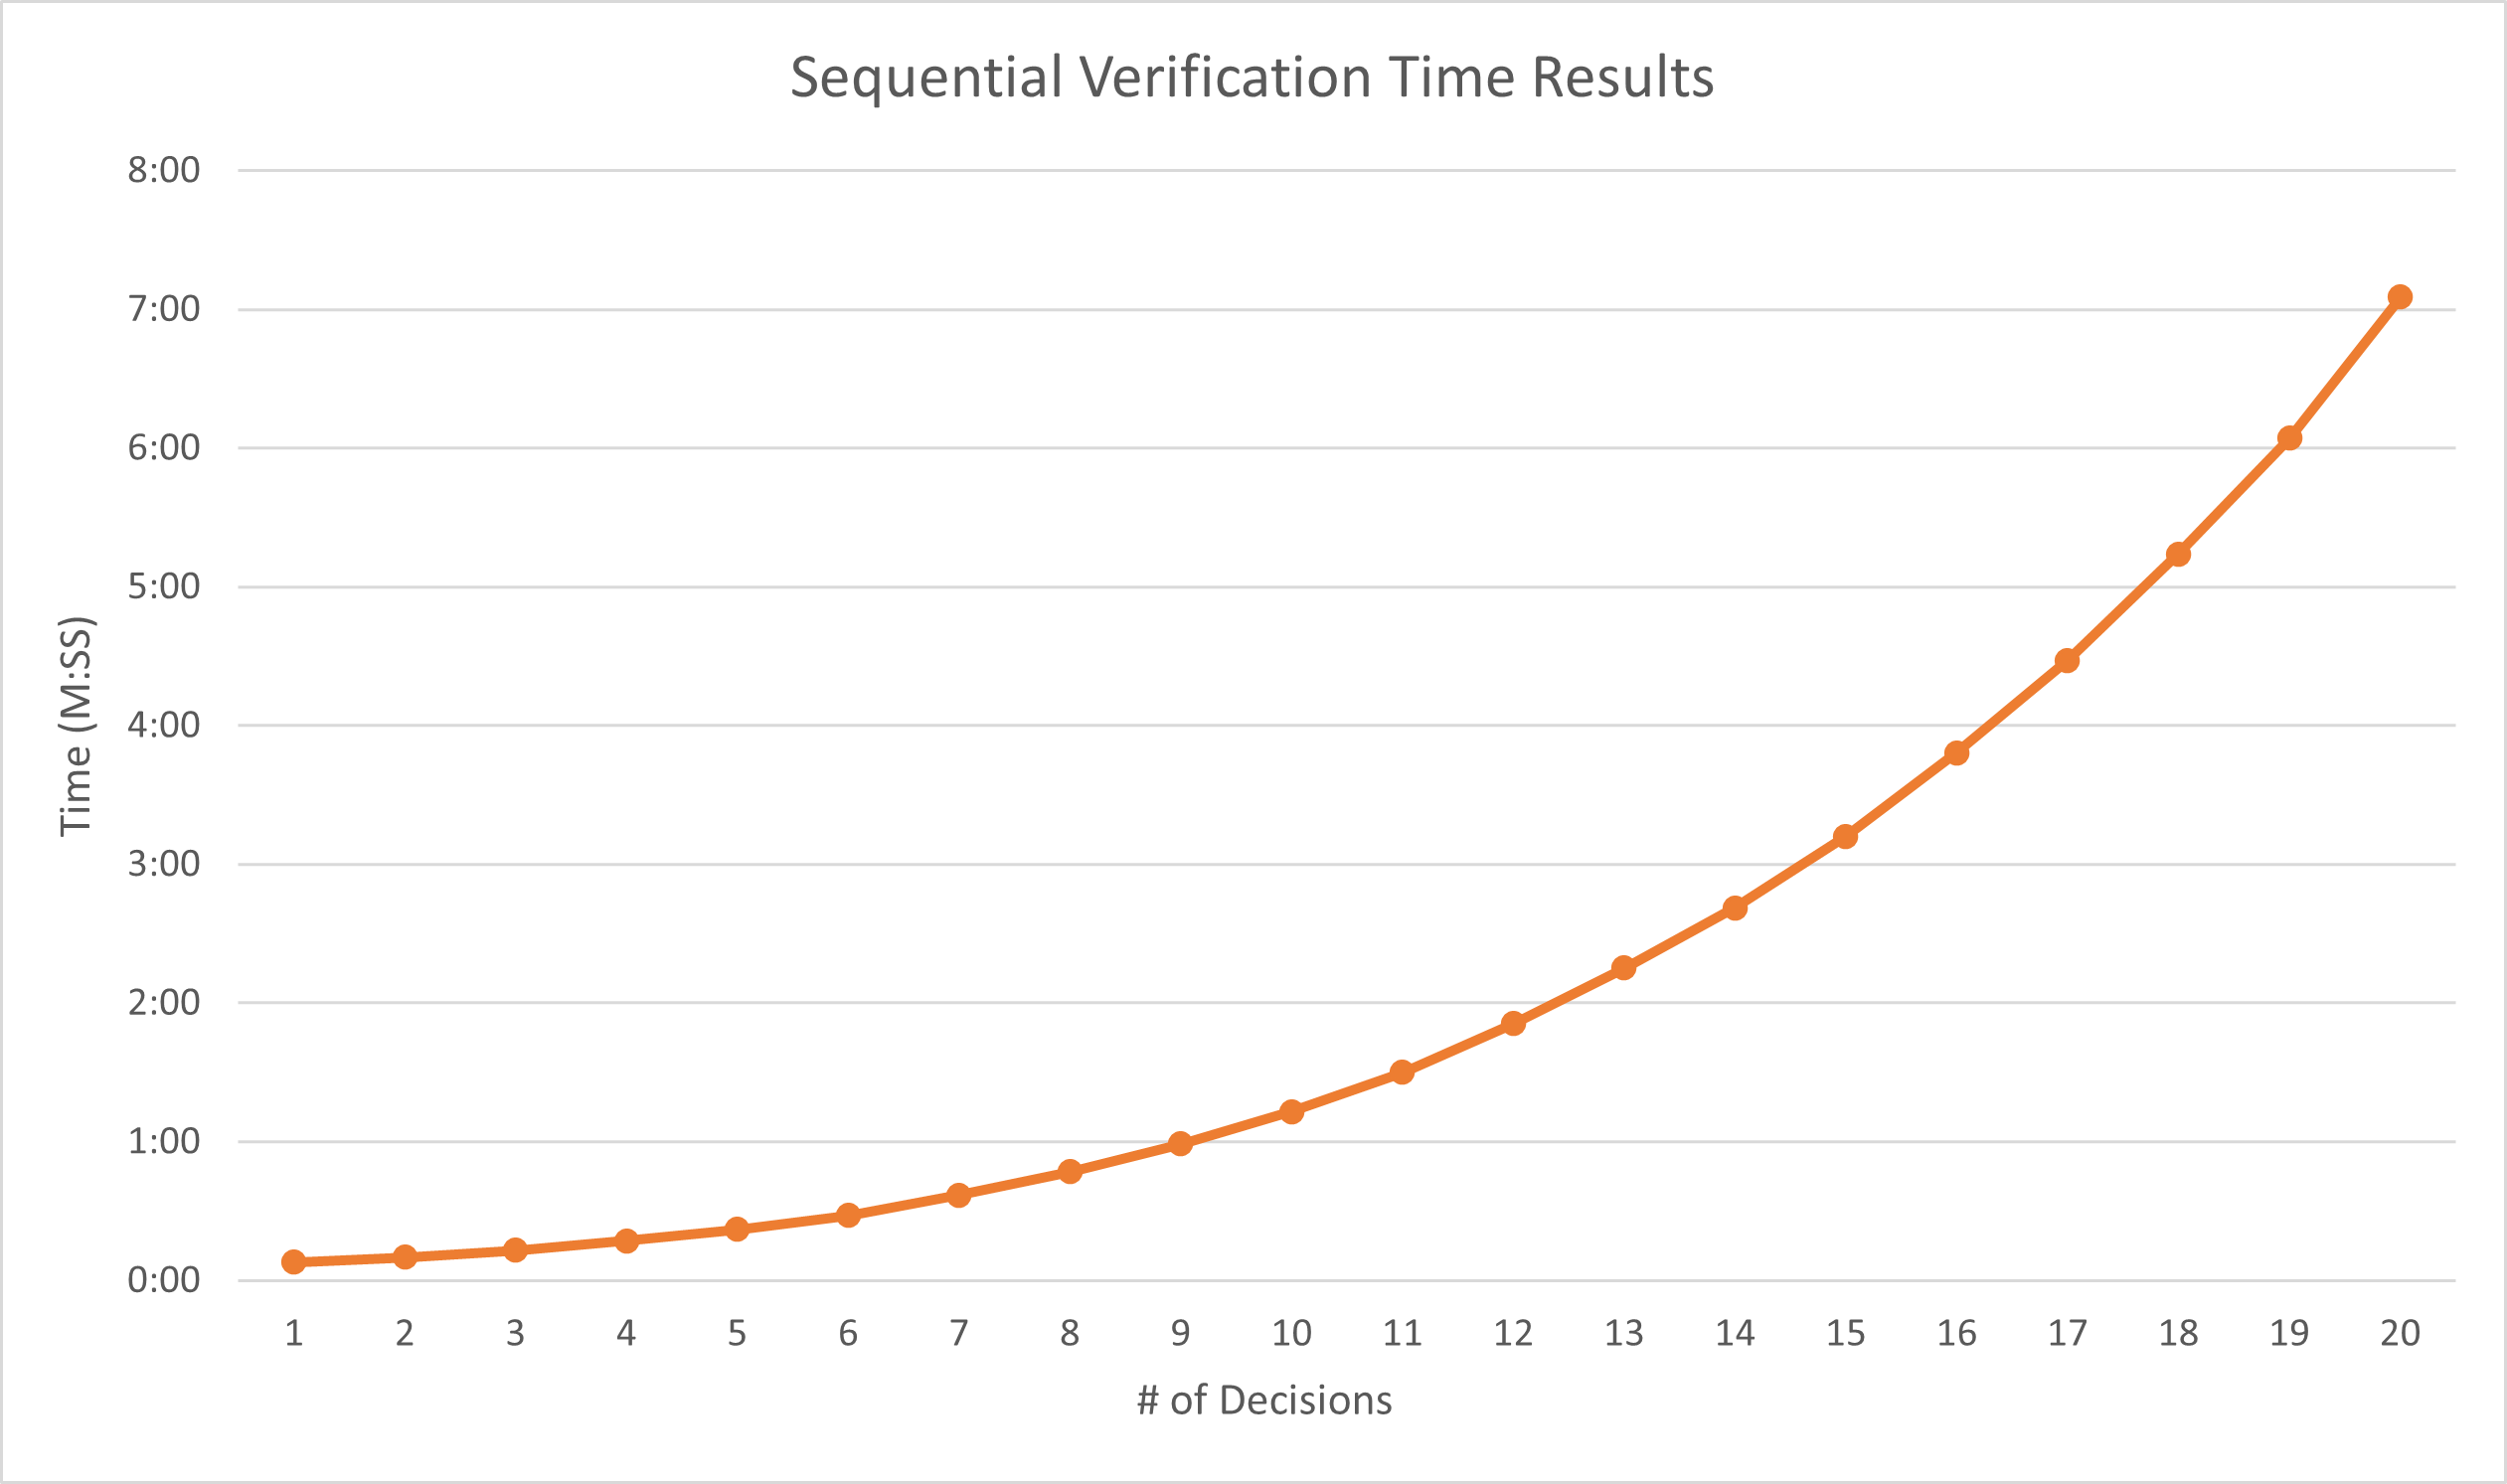
\includegraphics[width=\textwidth]{../figs/Data/Long_scaling_verification_times.png}
    \end{tabular}
  \end{center}
\caption{Verification times for the sequential scaling example by number of linear decisions}
\label{fig:longScalingVerificationTimes}
\end{figure*}

\figref{fig:wideScalingVerificationTimes} shows the increase in verification time as the number of synchronous actors increases in the parallel scaling BPMN example. Although the increase in verification time increases exponentially with the number of actors, it is important to note that this parallel example is the absolute worst case scenario in terms of parallelization. The structure of the parallel scaling example was created to introduce the maximum possible number of race conditions. This results in an incredibly fast increase in the number of states the model checker must search through.

In BPMN best practice, it is recommended to keep the number of parallel actors small in order to increase readability. Best practice often recommends subroutines and call activities in situations where a separate party is responsible for a large task. Short parallel tasks are not as significant because they result in considerably fewer race conditions as large tasks.

\begin{figure*}[t]
  \begin{center}
    \begin{tabular}{c}
        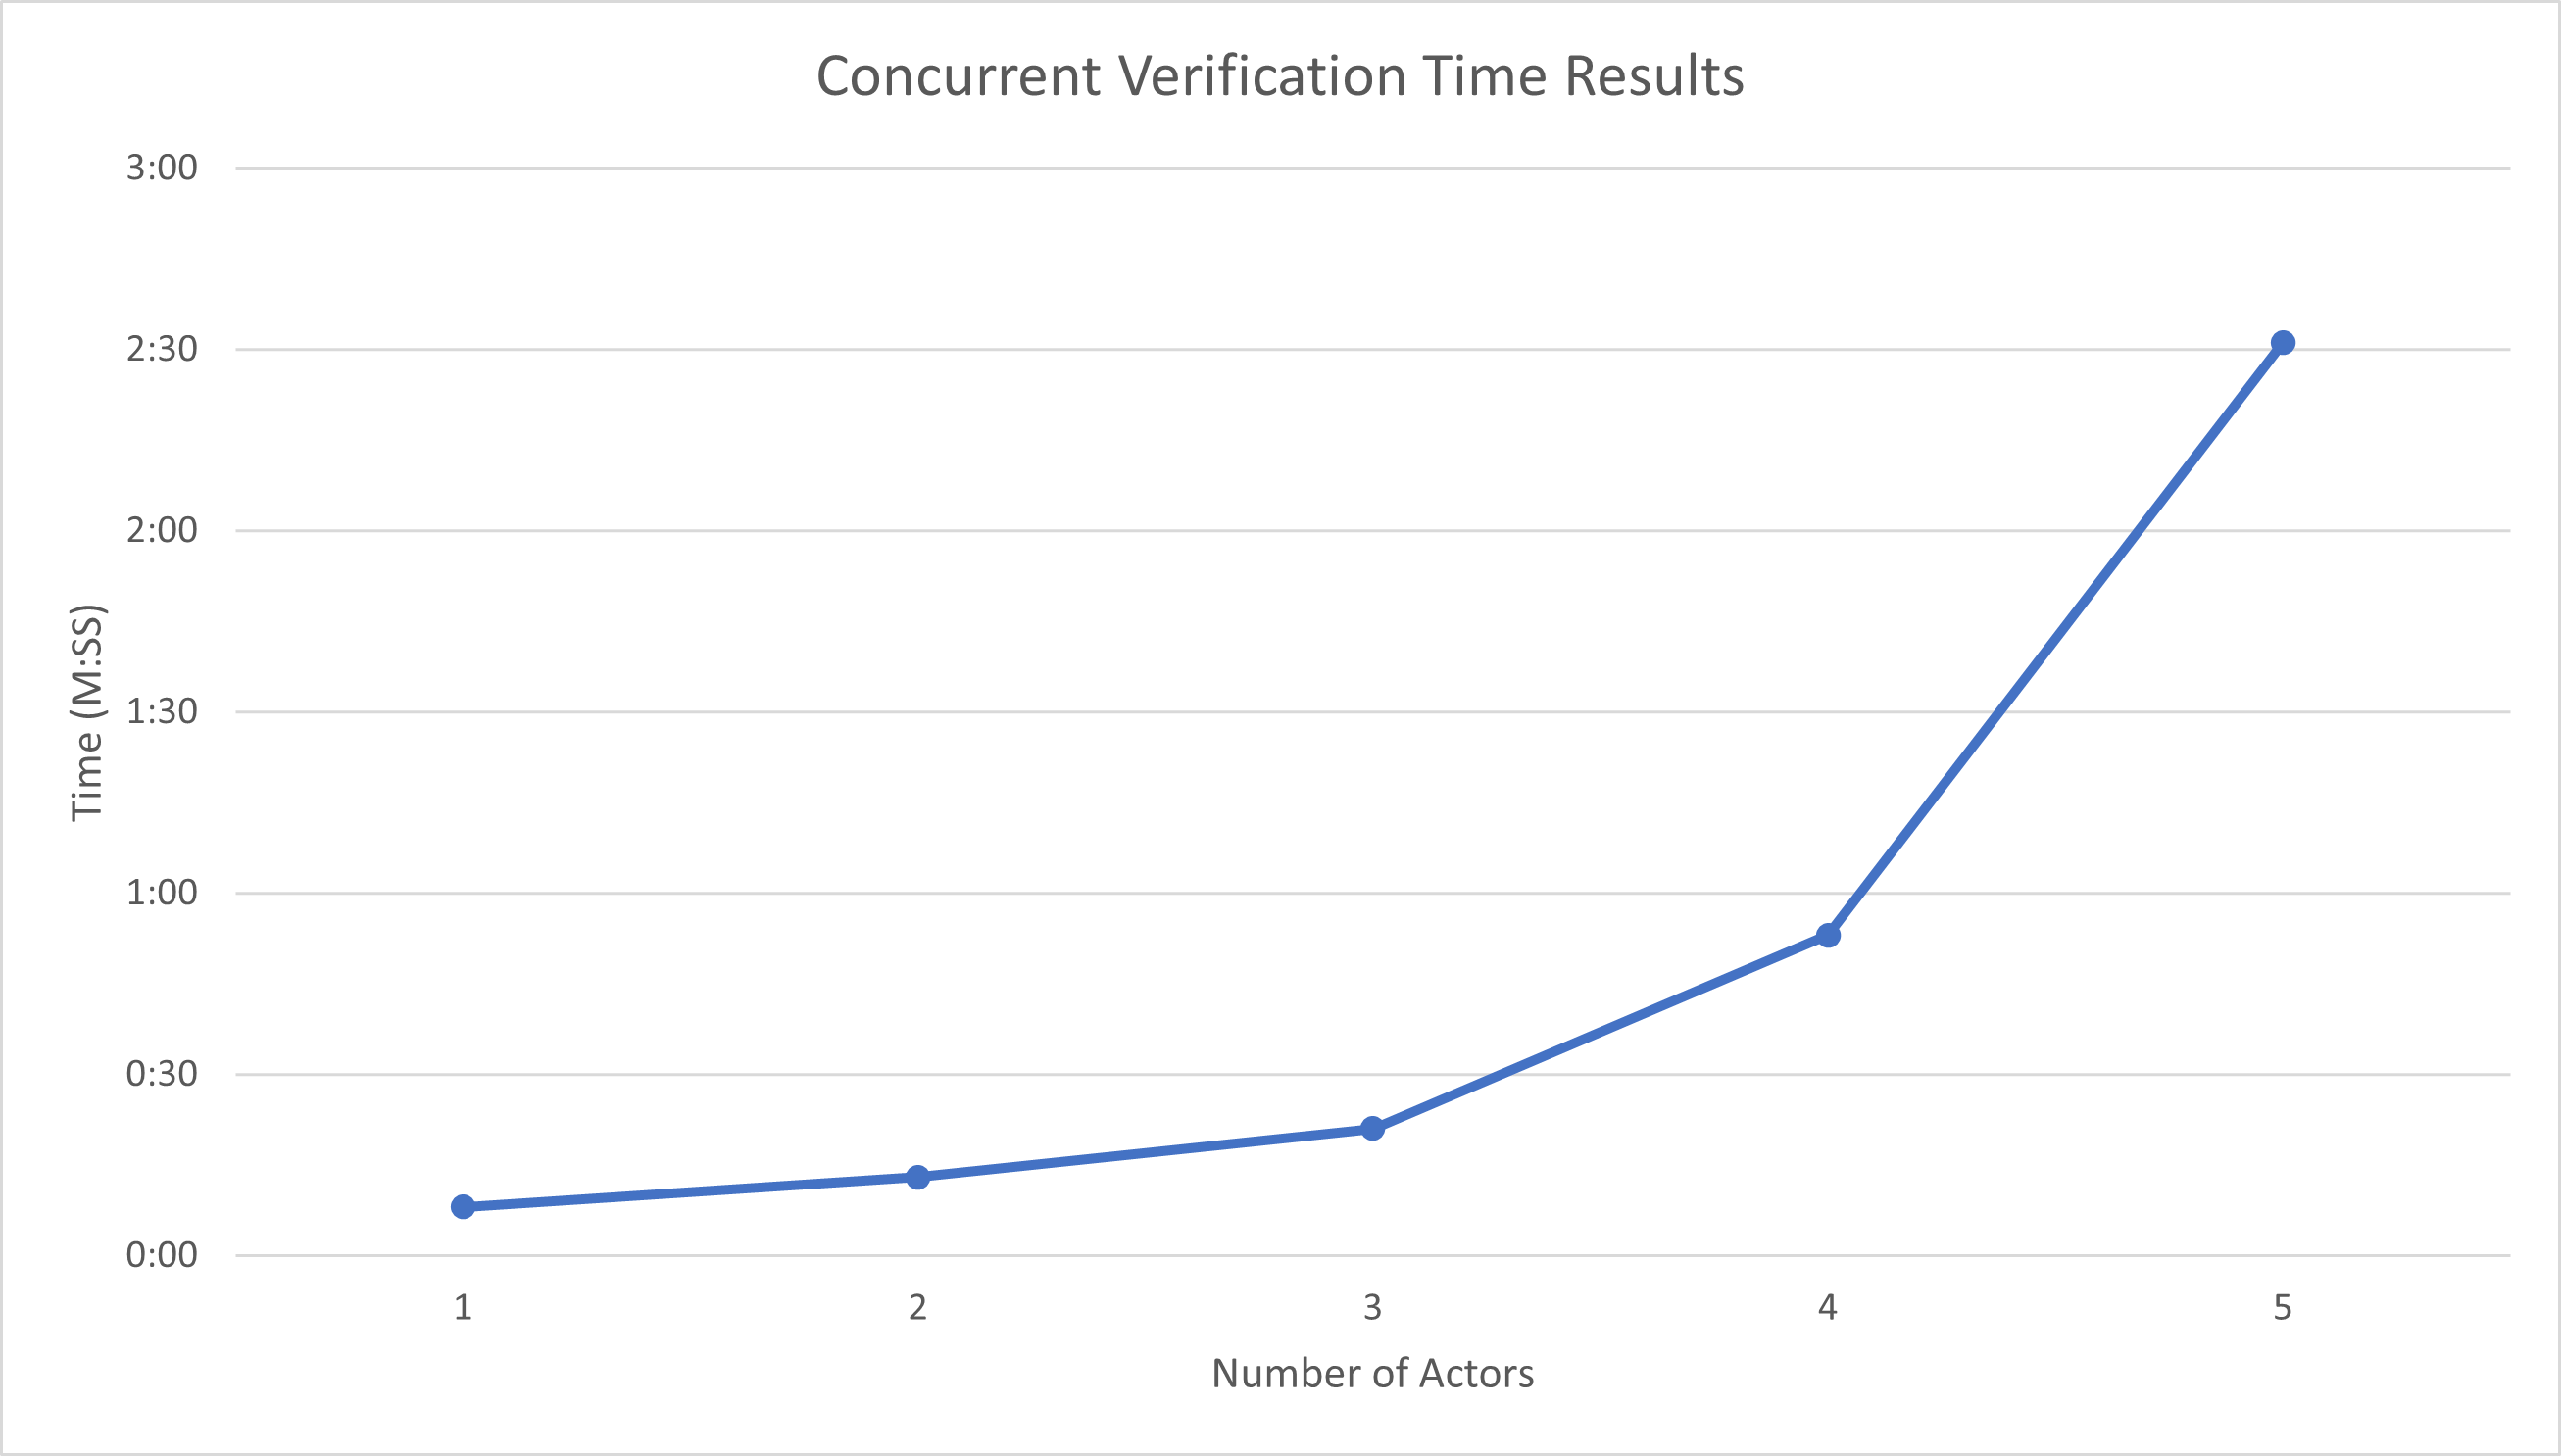
\includegraphics[width=\textwidth]{../figs/Data/Wide_scaling_verification_times.png}
    \end{tabular}
  \end{center}
\caption{Verification times for the parallel scaling example by number of concurrent actors}
\label{fig:wideScalingVerificationTimes}
\end{figure*}

.
.
.
.
.
.
.
.
.
.


\section{SPIN Verification Results}
\label{sec:results}
% The full Promela model, with the LTL properties for the CWP, is in a public Github repository \cite{repo}. 
% The \emph{README.md} file in the repository summarizes its content and how to verify the model. 
% The model is divided into three files: the CWP object state, the CWP LTL properties, and the BPMN workflow. A script, \emph{short-verify.sh}, combines the three files to create the Promela model and then runs SPIN on all the properties.

\begin{comment}
\begin{figure*}[t]
  \begin{center}
    \begin{tabular}{c}
      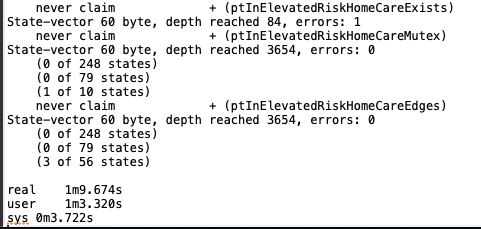
\includegraphics[scale=0.60]{../figs/proof-digest.png}
    \end{tabular}
  \end{center}
\caption{Some of the verification results from the SPIN model checker.}
\label{fig:proof}
\end{figure*}
The results for the state properties for \texttt{ptInElevatedRiskHomeCare} with the measured time verifying the entire model is shown in \figref{fig:proof}.
\end{comment}

\begin{comment}
As a reminder, the model and properties can be found at \cite{repo}.
Verification takes three to four minutes on an Intel Core i7 laptop with 16 Gb of RAM. It does not tax the system in any way.
All the existential properties (i.e., the properties ending with \emph{Exists}) resulted in an error. The error is the existential witness.
All other properties pass with no errors. The script's output includes not just the error report but the coverage summary of the processes and properties.
The first two entries pertain to the clinician and patient-caregiver processes. There should never be uncovered states in these processes.
Uncovered states means that there are unreachable behaviors in the model---not good. The third entry is the property being verified.
It is not unusual to have uncovered states here when there is no reported error since the error behavior is not found in the model---good.

To illustrate the value of model checking during design, it found many subtle errors during BPMN development.
Also in an early version of the CWP, SPIN found a trace through the workflow where the patient expires while in appropriate home care which is not allowed by the CWP. The error was in the CWP because the meaning of appropriate home care was not precise. It omitted information about trending severity that would indicate an elevated risk. The domain experts reviewed and approved changes to the transition conditions in the CWP, and SPIN then verified that the workflow preserved the property that patients only expire in elevated risk or in the hospital under those changed conditions. The very act of verifying the workflow against the CWP, even assuming the CWP is correct, yields important insights that are easily missed by manual inspection with domain experts.
\end{comment}




\section{Related Work}
\begin{comment}
It is possible to translate live sequence charts to LTL \cite{KUMAR, KUMAR2009137}. These translations result in large intractable formulas whereas the work here creates several connected small formulas that are easy for SPIN. UML modeling uses \emph{synchronous observer automata} to encode and verify safety properties \cite{8906967}. The CWP can be thought of as a synchronous observer, and it is possible to express it in SPIN for safety verification, but that complicates existential properties and may result in a larger state space. Other work verifies that UML state diagrams implement their associated activity diagrams (workflows) with the NuSMV model checker \cite{7436156}. The workflows are turned into LTL, just opposite of the work here. That said, it is possible to extract a CWP from workflow models, in which case the intent is to discover what the system will accomplish.

There is some work related in translating models in the \emph{Business Process Execution Language} (BPEL) to Promela \cite{bpelToPromela}. The semantics are different and is limited in scope to web-services. BPMN choreographies have been modeled in Promela and verified with SPIN for deadlock, but choreographies ignore workflows and only model message sequencing \cite{choreography}. The translation of BPMN to Promela is inspired by existing methods for turning Petri Nets into equivalent Promela models \cite{petrinetToPromela, petrinetInspiration}. These however do not include data. The translation in this paper is also based off of early prototype translations of BPMN to Promela using message channels for synchronization \cite{bpmn2promela} whereas the translation here uses global variables to mitigate state explosion.
\end{comment}

\section{Conclusions and Future Work}
\begin{comment}

The CWP was coupled with workflow models to create a verification problem suitable for the SPIN model checker. This was accomplished by translating the CWP into an set of LTL properties that together express the same meaning as the CWP. The workflow models can be directly turned into equivalent models in Promela, the input language to SPIN, which is able to prove whether the workflows correctly implement the CWP. Such mechanized and automated reasoning is critical to assurance that the design of a complex distributed system is capable to establish and maintain \emph{actionable risk awareness}. 

The CWP defines thresholds of patient risk during home care and their appropriate actions, thereby making a clear connection from the verified design to its larger, societal purpose of safe care. The interaction between users and AI is only modestly complex, however it strikes the balance needed to illustrate the method with an example workflow that can be followed by readers without much BPMN familiarity. 
The complexity should increase when deployment collects confirmation/dismissal of alerts, and eventual patient outcomes, for AI machine learning to increase alert precision.

Our approach's generality depends on discovery and modeling CWPs. Prior to model-checking CWPs their principles  were applied to human-computer integration for highly usable designs of integrated aircraft mission and maintenance scheduling \cite{workcentered}, joint U.S.-Russia maneuver planning for the \emph{International Space Station}  \cite{10.1145/1978942.1979311}, and health care coordination \cite{BERRY201615}. These CWPs define fundamental requirements for systems that must respond to events outside their direct control. The principles of CWP were recently adopted in the SysML v.2 standard.

Model-checking scalability depends on workflows' number of asynchronous actors, synchronization points, etc. BPMN supports hierarchies of sub-processes for larger workflows, where CWPs may be defined for each; regardless, the case study is a key step towards automation. 

Our current research aims to automate CWP translation to LTL, and BPMN to Promela, so counter-examples from SPIN point directly to CWPs. This undertaking is a non-trivial engineering task as model checking requires domain expertise and the counter-examples produced by SPIN are infinite by virtue of LTL semantics. Ongoing efforts are refining the SPIN translations to include additional global states that correspond directly to CWP states and edges to simplify counter-example mapping. 

Other research under consideration could explore reuse of verified designs in watcher systems that monitor their deployed implementations. CWP models could also be used to derive efficiency measures, e.g., reducing the amount of activity that does not advance the CWP states could be a new approach to efficiency.  

The focus of conventional design methods is on software, which leaves important aspects of system success largely to chance. 
This paper's novel contribution is verifiable integration of human-computer teaming on cognitive tasks. 
The need is industry-wide. 
Expected benefits of verifiable integration include greater safety and reliability of systems for many other critical domains. 

\end{comment}

Workflows have become a regular tool in modern business practices. They have also been increasingly used in the field of LC/NC development. But the efforts to verify workflow execution have been lacking. 

In this paper, we showed that workflows can be translated into verifiable Promela code. That code can then be verified against LTL properties represented by CWPs. This process can and has been automated, and we have provided an implementation for performing automated translation. Our solution uses an intermediate python graph structure and a visitor pattern to generate the Promela model and LTL properties. Additionally, we improve upon the format of the verification results by providing step-by-step annotated images when a verification error occurs. This improvement speeds up and eases the incremental process of modeling correct workflows.

The automated process of verifying BPMN workflows has been tested on three examples as case-studies and two more as scalability exercises. The results show that this method of automated model checking is viable for sizes of workflows frequently seen in LC/NC applications.

There are improvements to be made to the methods described in this paper. First, there should be efforts to conduct a usability study of the automation tool. We are interested not only in the ease of verification, but also in the generated Promela model's readability. Additionally, a usability study should seek to understand the usability of the generated counterexample in finding and fixing BPMN errors.

There should be an effort to further automate the identification of the behavior models. Currently, the behavior models must be manually written by an expert in the workflow's domain. It is our desire that the majority of the behavior models be inferred from different aspects of the BPMN itself. An iterative verification approach could be used: Auto-generated behavior models are tested through verification. After each iteration, verification results are analyzed and behavior models are modified. Additional tools such as AI might also be utilized.

There might also be efforts to explore additional verification properties of interest. For example, there may be a property that enforces eventual existence of valid end states in the BPMN. It may be the case that the BPMN accomplishes the work in the CWP before it reaches an end state itself. This might be undesirable behavior depending on the context.

In order to be usable on many commercial workflows, the tool will need to support many new BPMN elements, especially sub-tasks and call activities. For each of these, there should be support for hierarchical verification. Essentially, the sub-task should be verified independently to behave in the desired way, with its own associated CWP. Then, once we are confident it behaved that way, we can assume that behavior in the behavior models of the parent BPMN workflow. This process has not been implemented into the verification tool at this time.

We would like to compile a larger set of practical test inputs in order to get a more complete view of the tool's limitations and commercial viability. Commercial best modeling practices indicate that workflow scale should not cause problems for the automation tool, but having a large set of working examples would still be desirable.

There may be more effective alternative ways of representing the verification properties. Currently, we are representing them as LTL properties which are supported natively by the model checker we use, SPIN. It may be more efficient, however, to generate never claims directly, since SPIN internally converts each LTL property into never claims anyway.


\section*{Acknowledgment}
\addcontentsline{toc}{section}{Acknowledgment}

\bibliographystyle{IEEEtran}
{\small 
\bibliography{bibliography}}

\end{document}
